\begin{frame}{Detección de movimientos en un tablero de ajedrez \footnotemark}
%\begin{block}{Detección de movimientos en un tablero de ajedrez \footnotemark} 
\begin{columns}
\begin{column}{0.38\textwidth}
Aplicación de escritorio:
	\begin{itemize}
\item Entorno semicontrolado con una cámara y una Laptop con OpenCV
\item Detecta las esquinas del tablero de ajedrez
\item Transformada de Hough
\item Detectar si hay casilla o no dentro de la región de interés
	\end{itemize}
\end{column}
\begin{column}{0.28\textwidth}
\begin{center}
     %%%%% this is a minipage, so \textwidth is already adjusted to the size of the column
     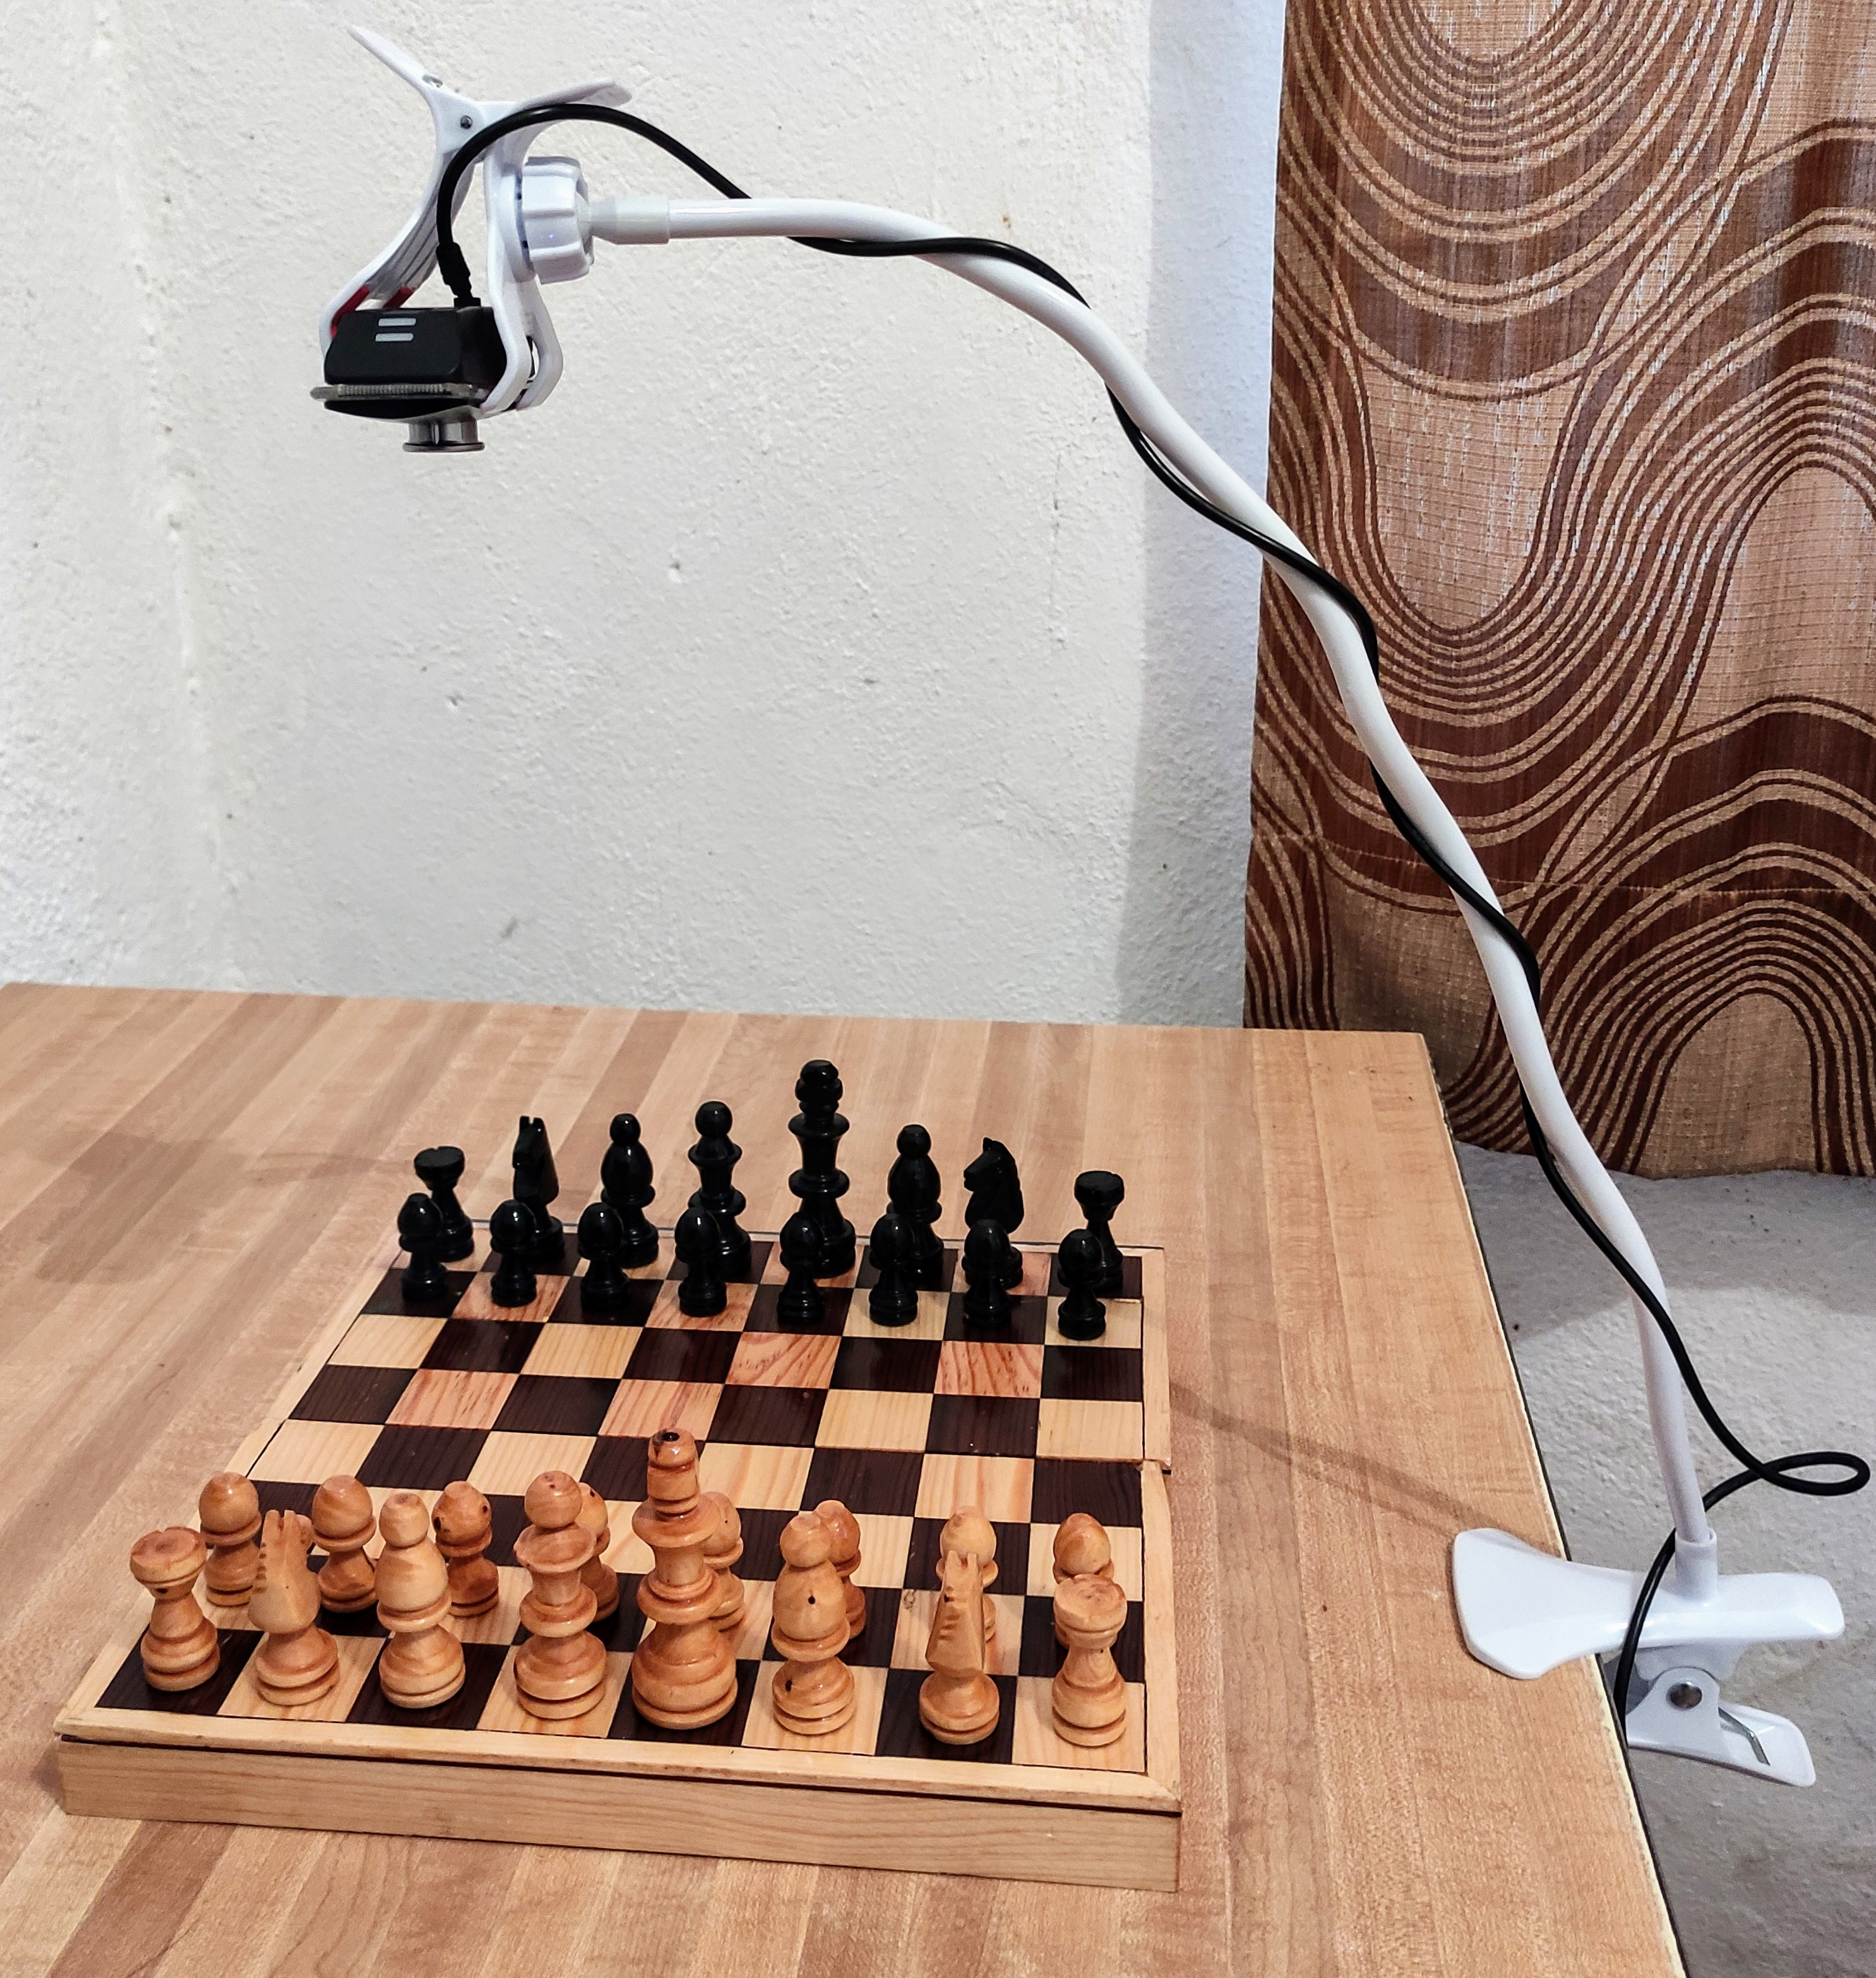
\includegraphics[width=0.75\textwidth]{Figs/AjedrezFroylan1}\\
%     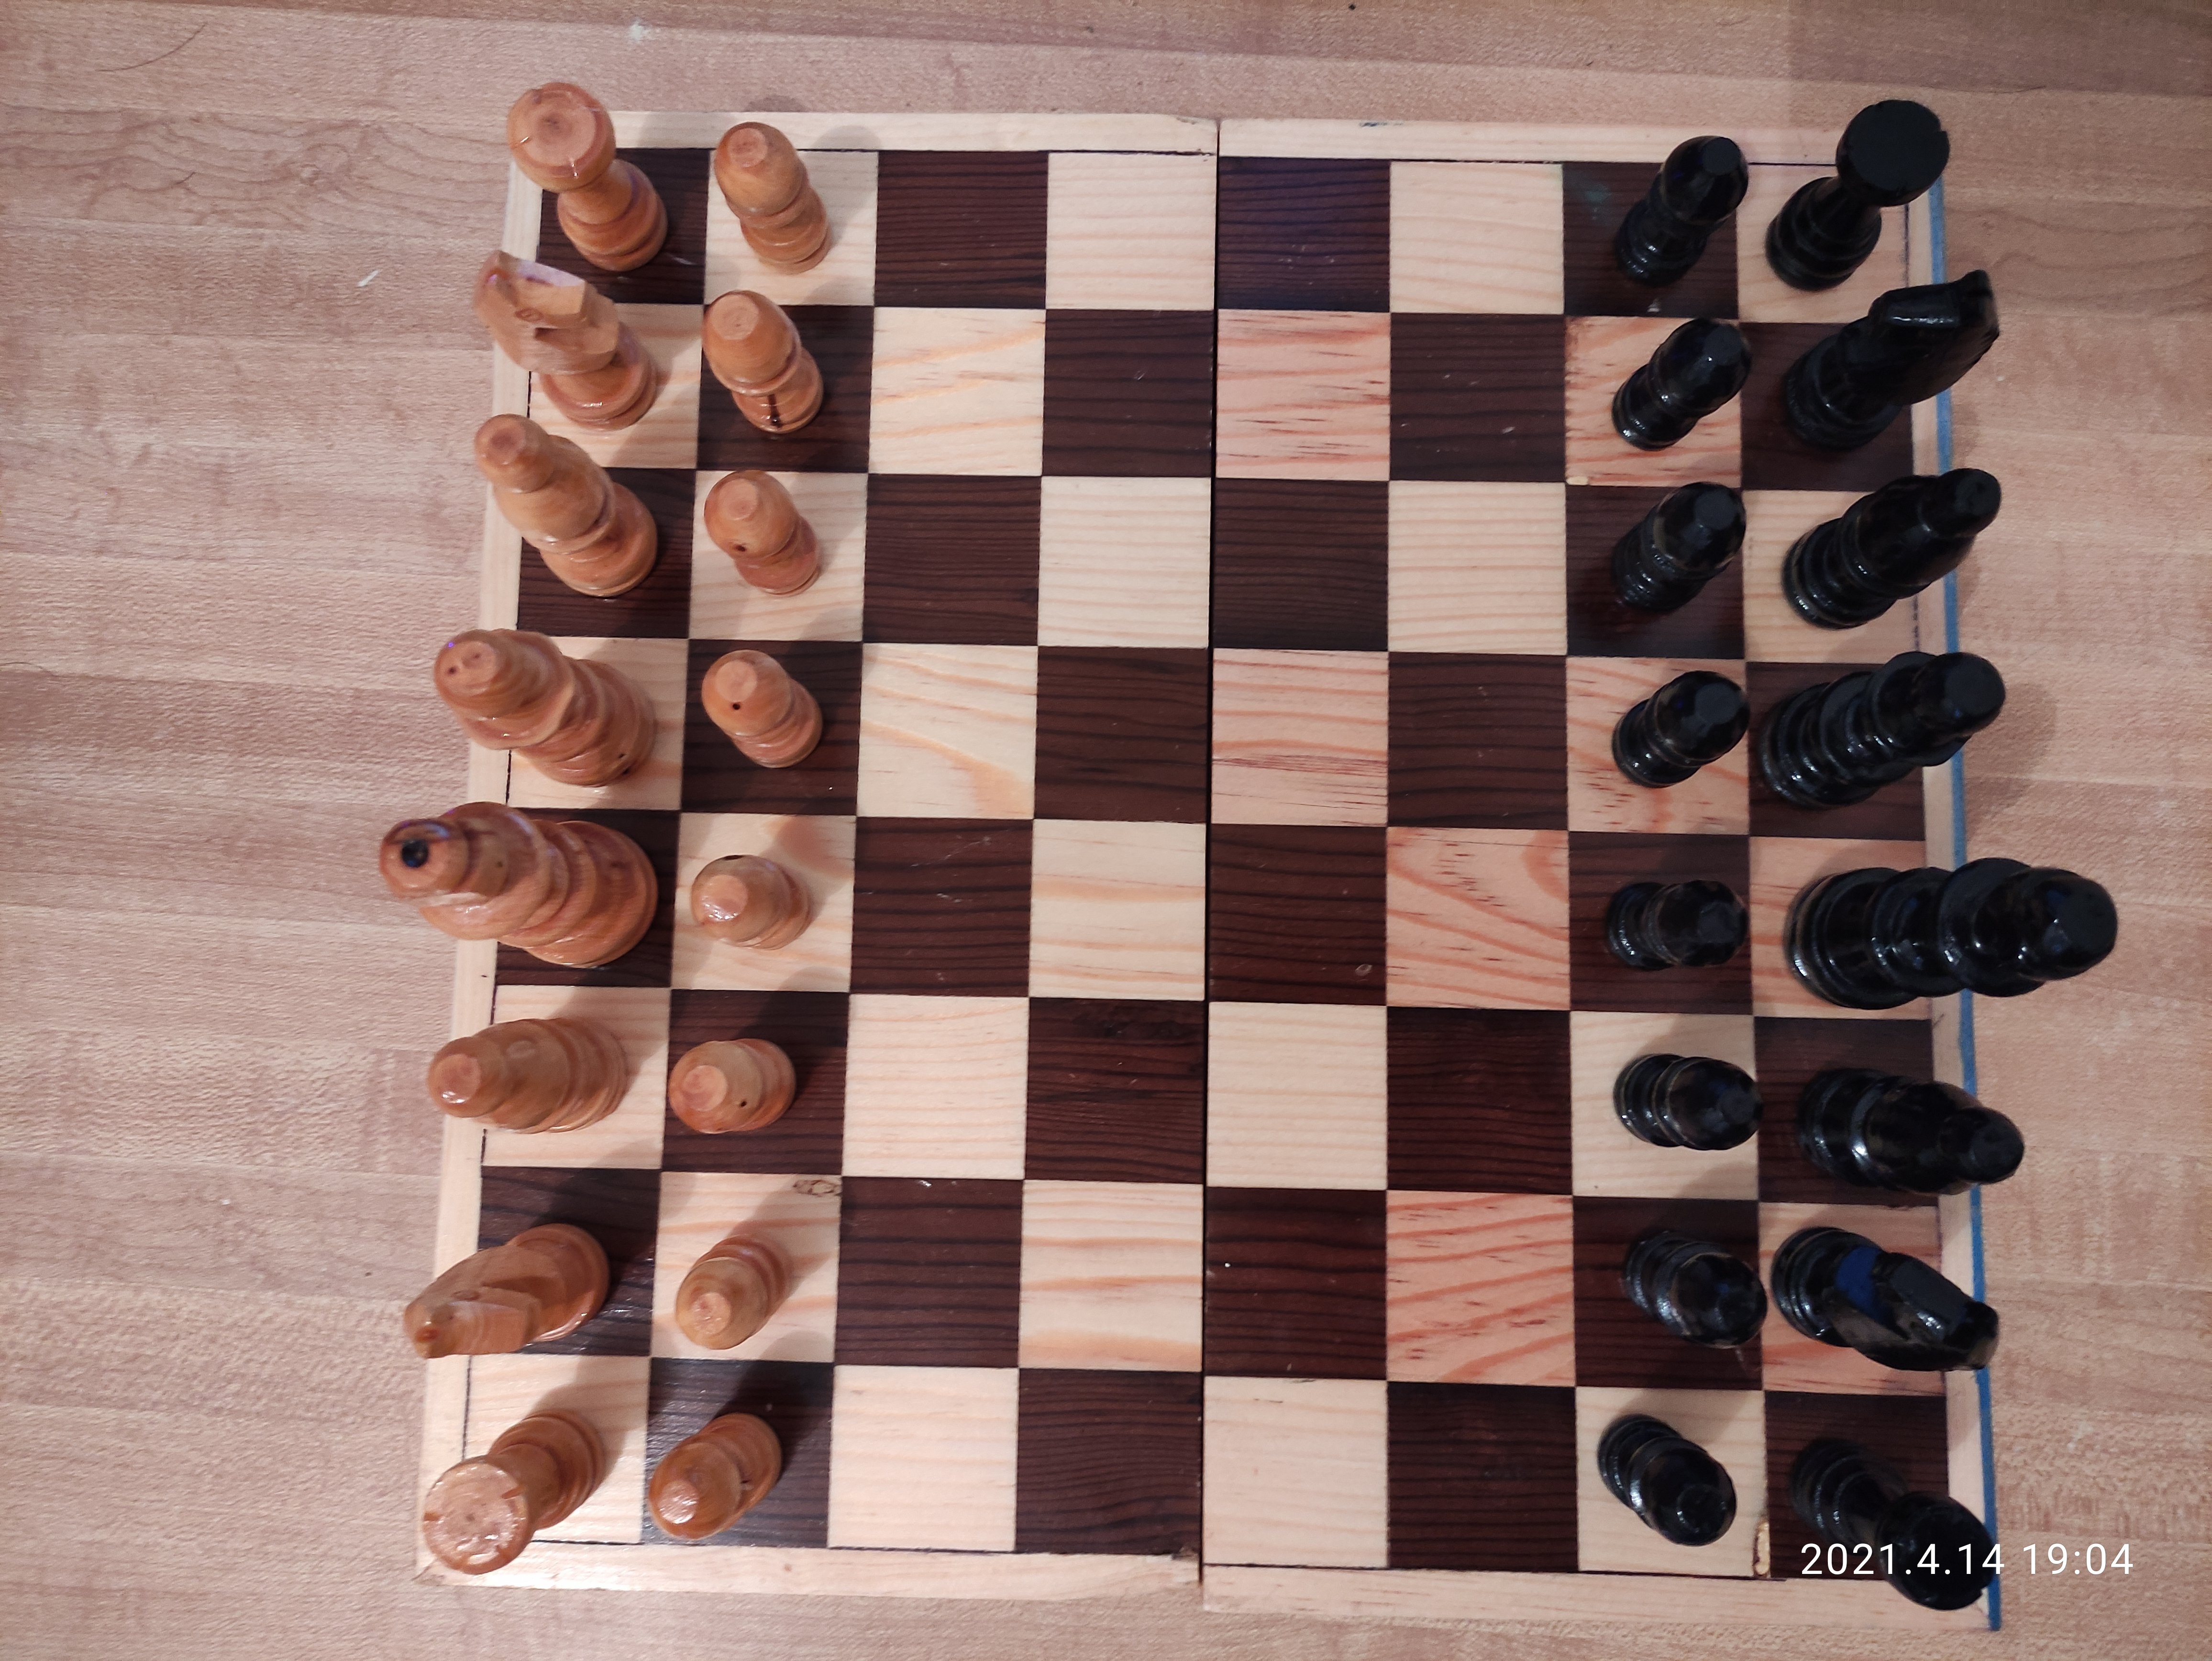
\includegraphics[width=0.35\textwidth]{Figs/AjedrezFroylan2}
     \end{center}
\end{column}
\begin{column}{0.28\textwidth}
\begin{center}
     %%%%% this is a minipage, so \textwidth is already adjusted to the size of the column
 %    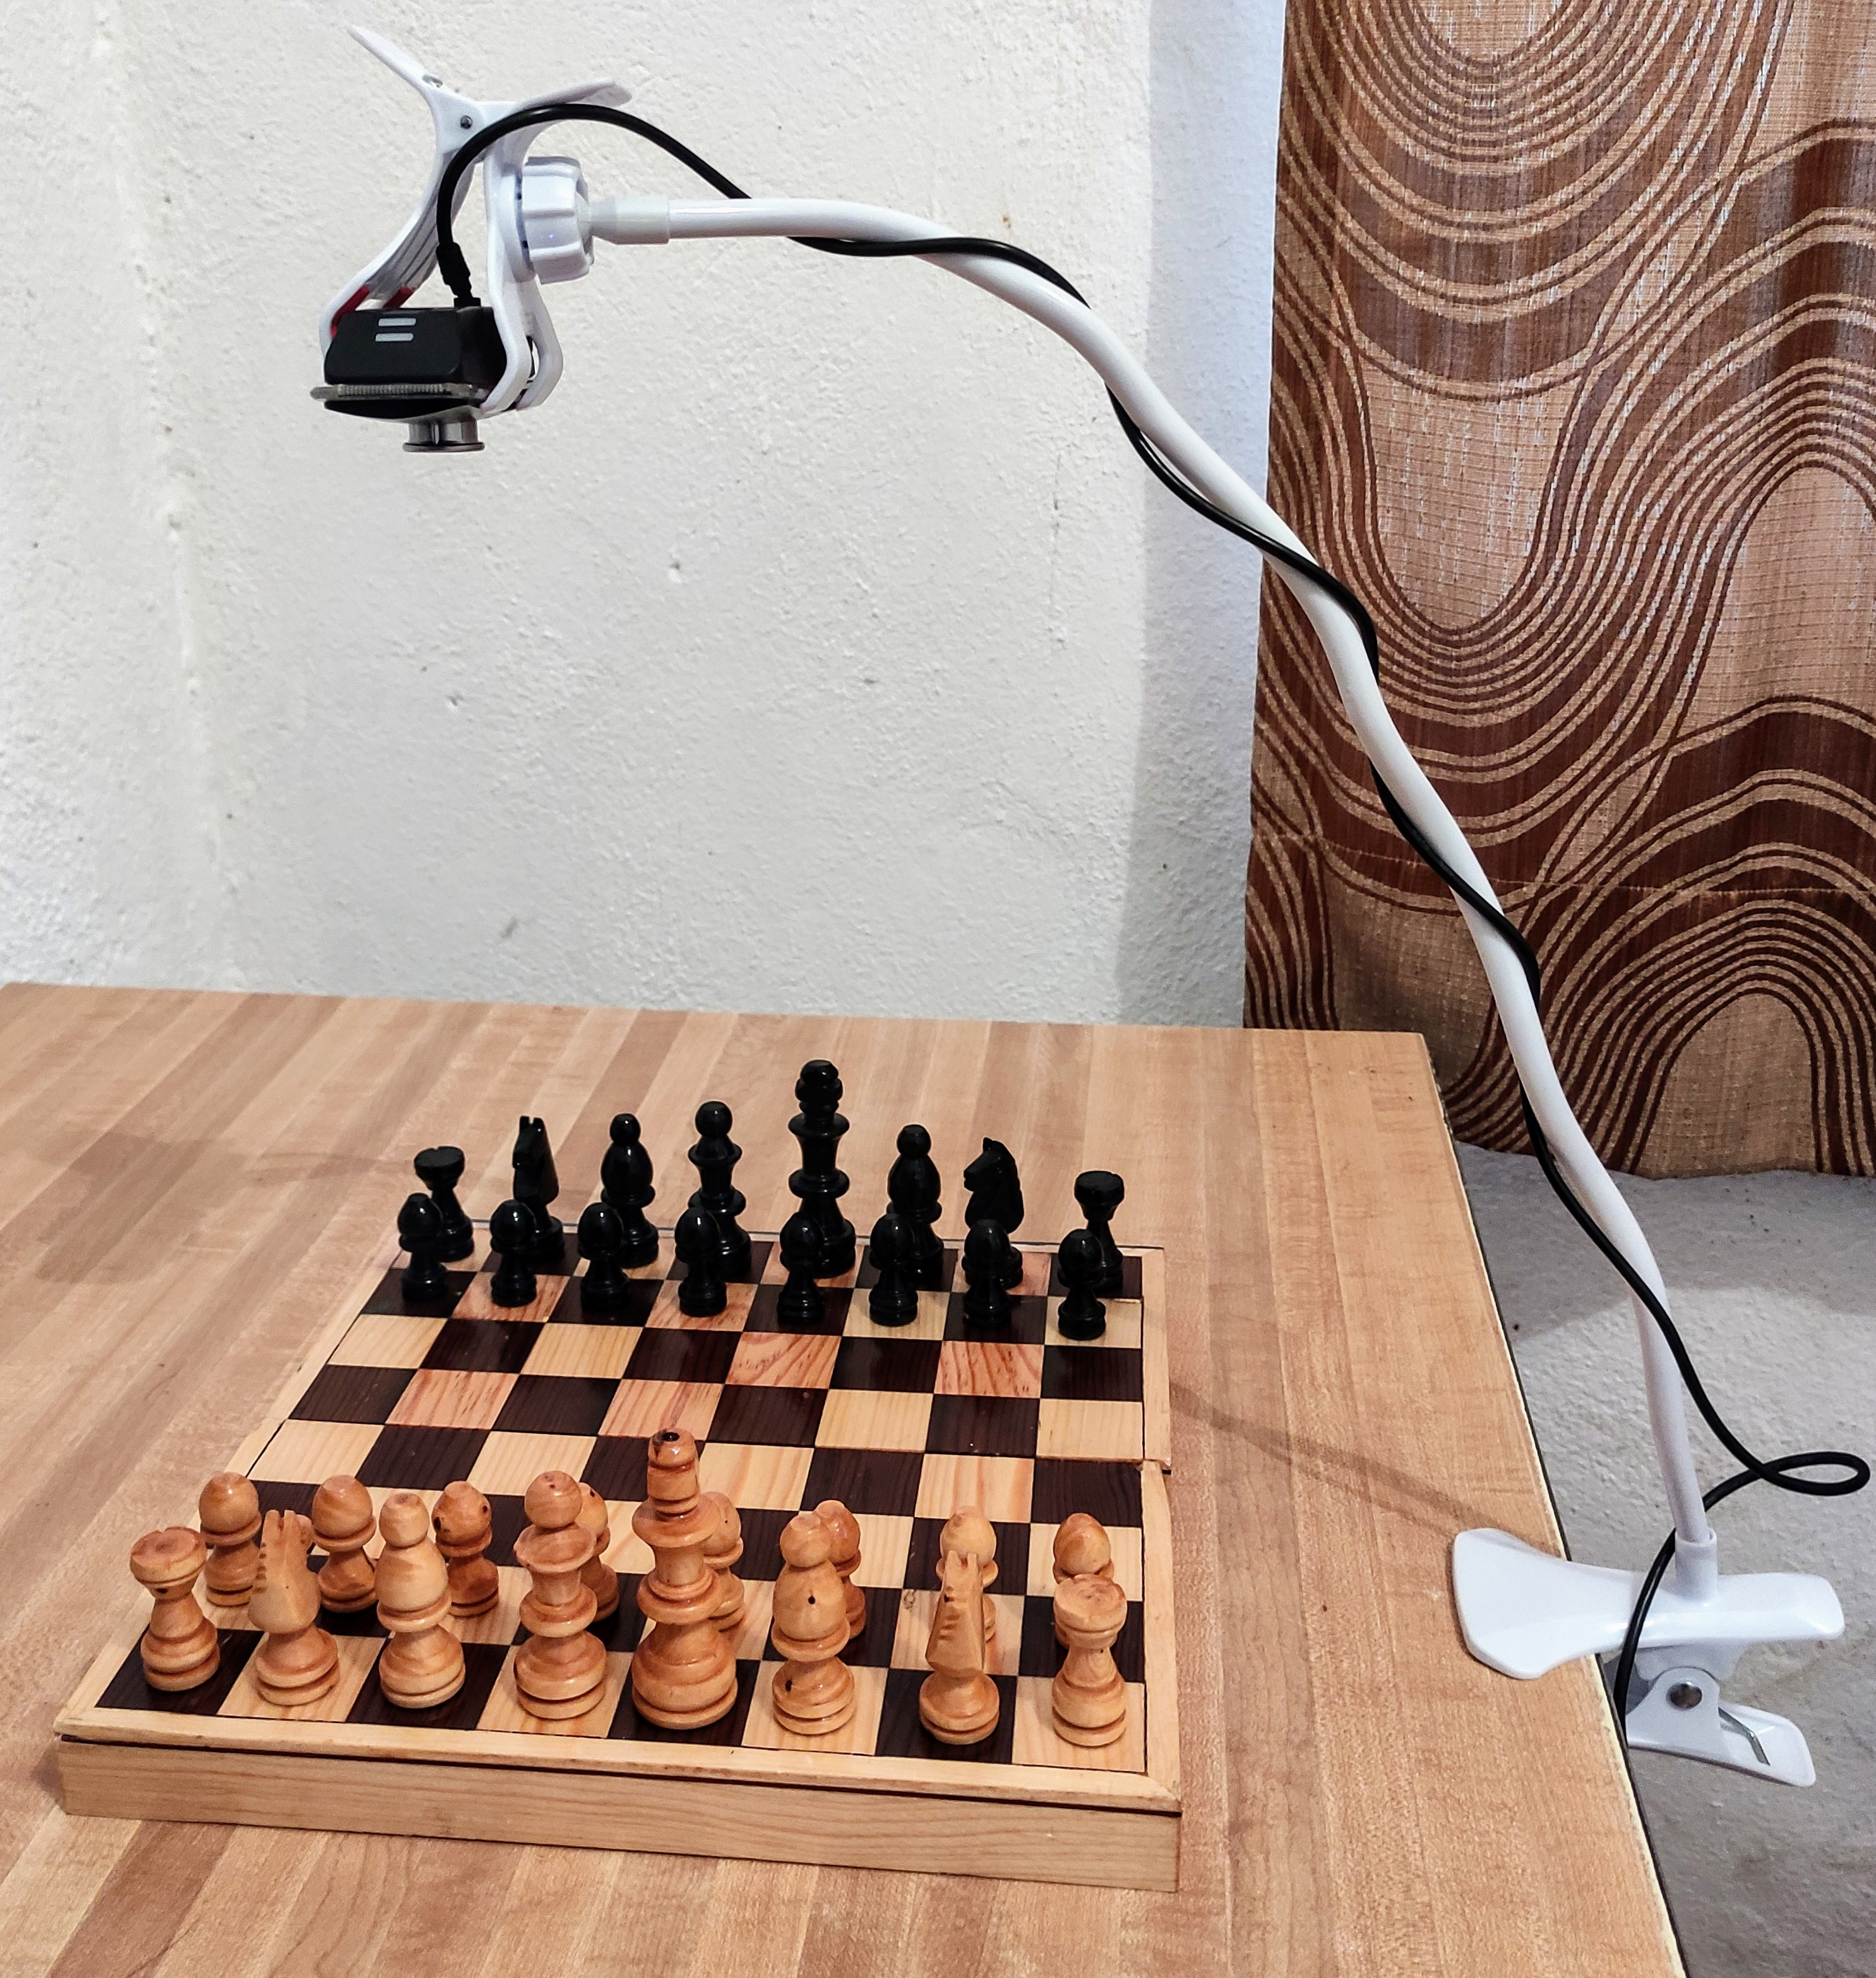
\includegraphics[width=0.35\textwidth]{Figs/AjedrezFroylan1}\\
     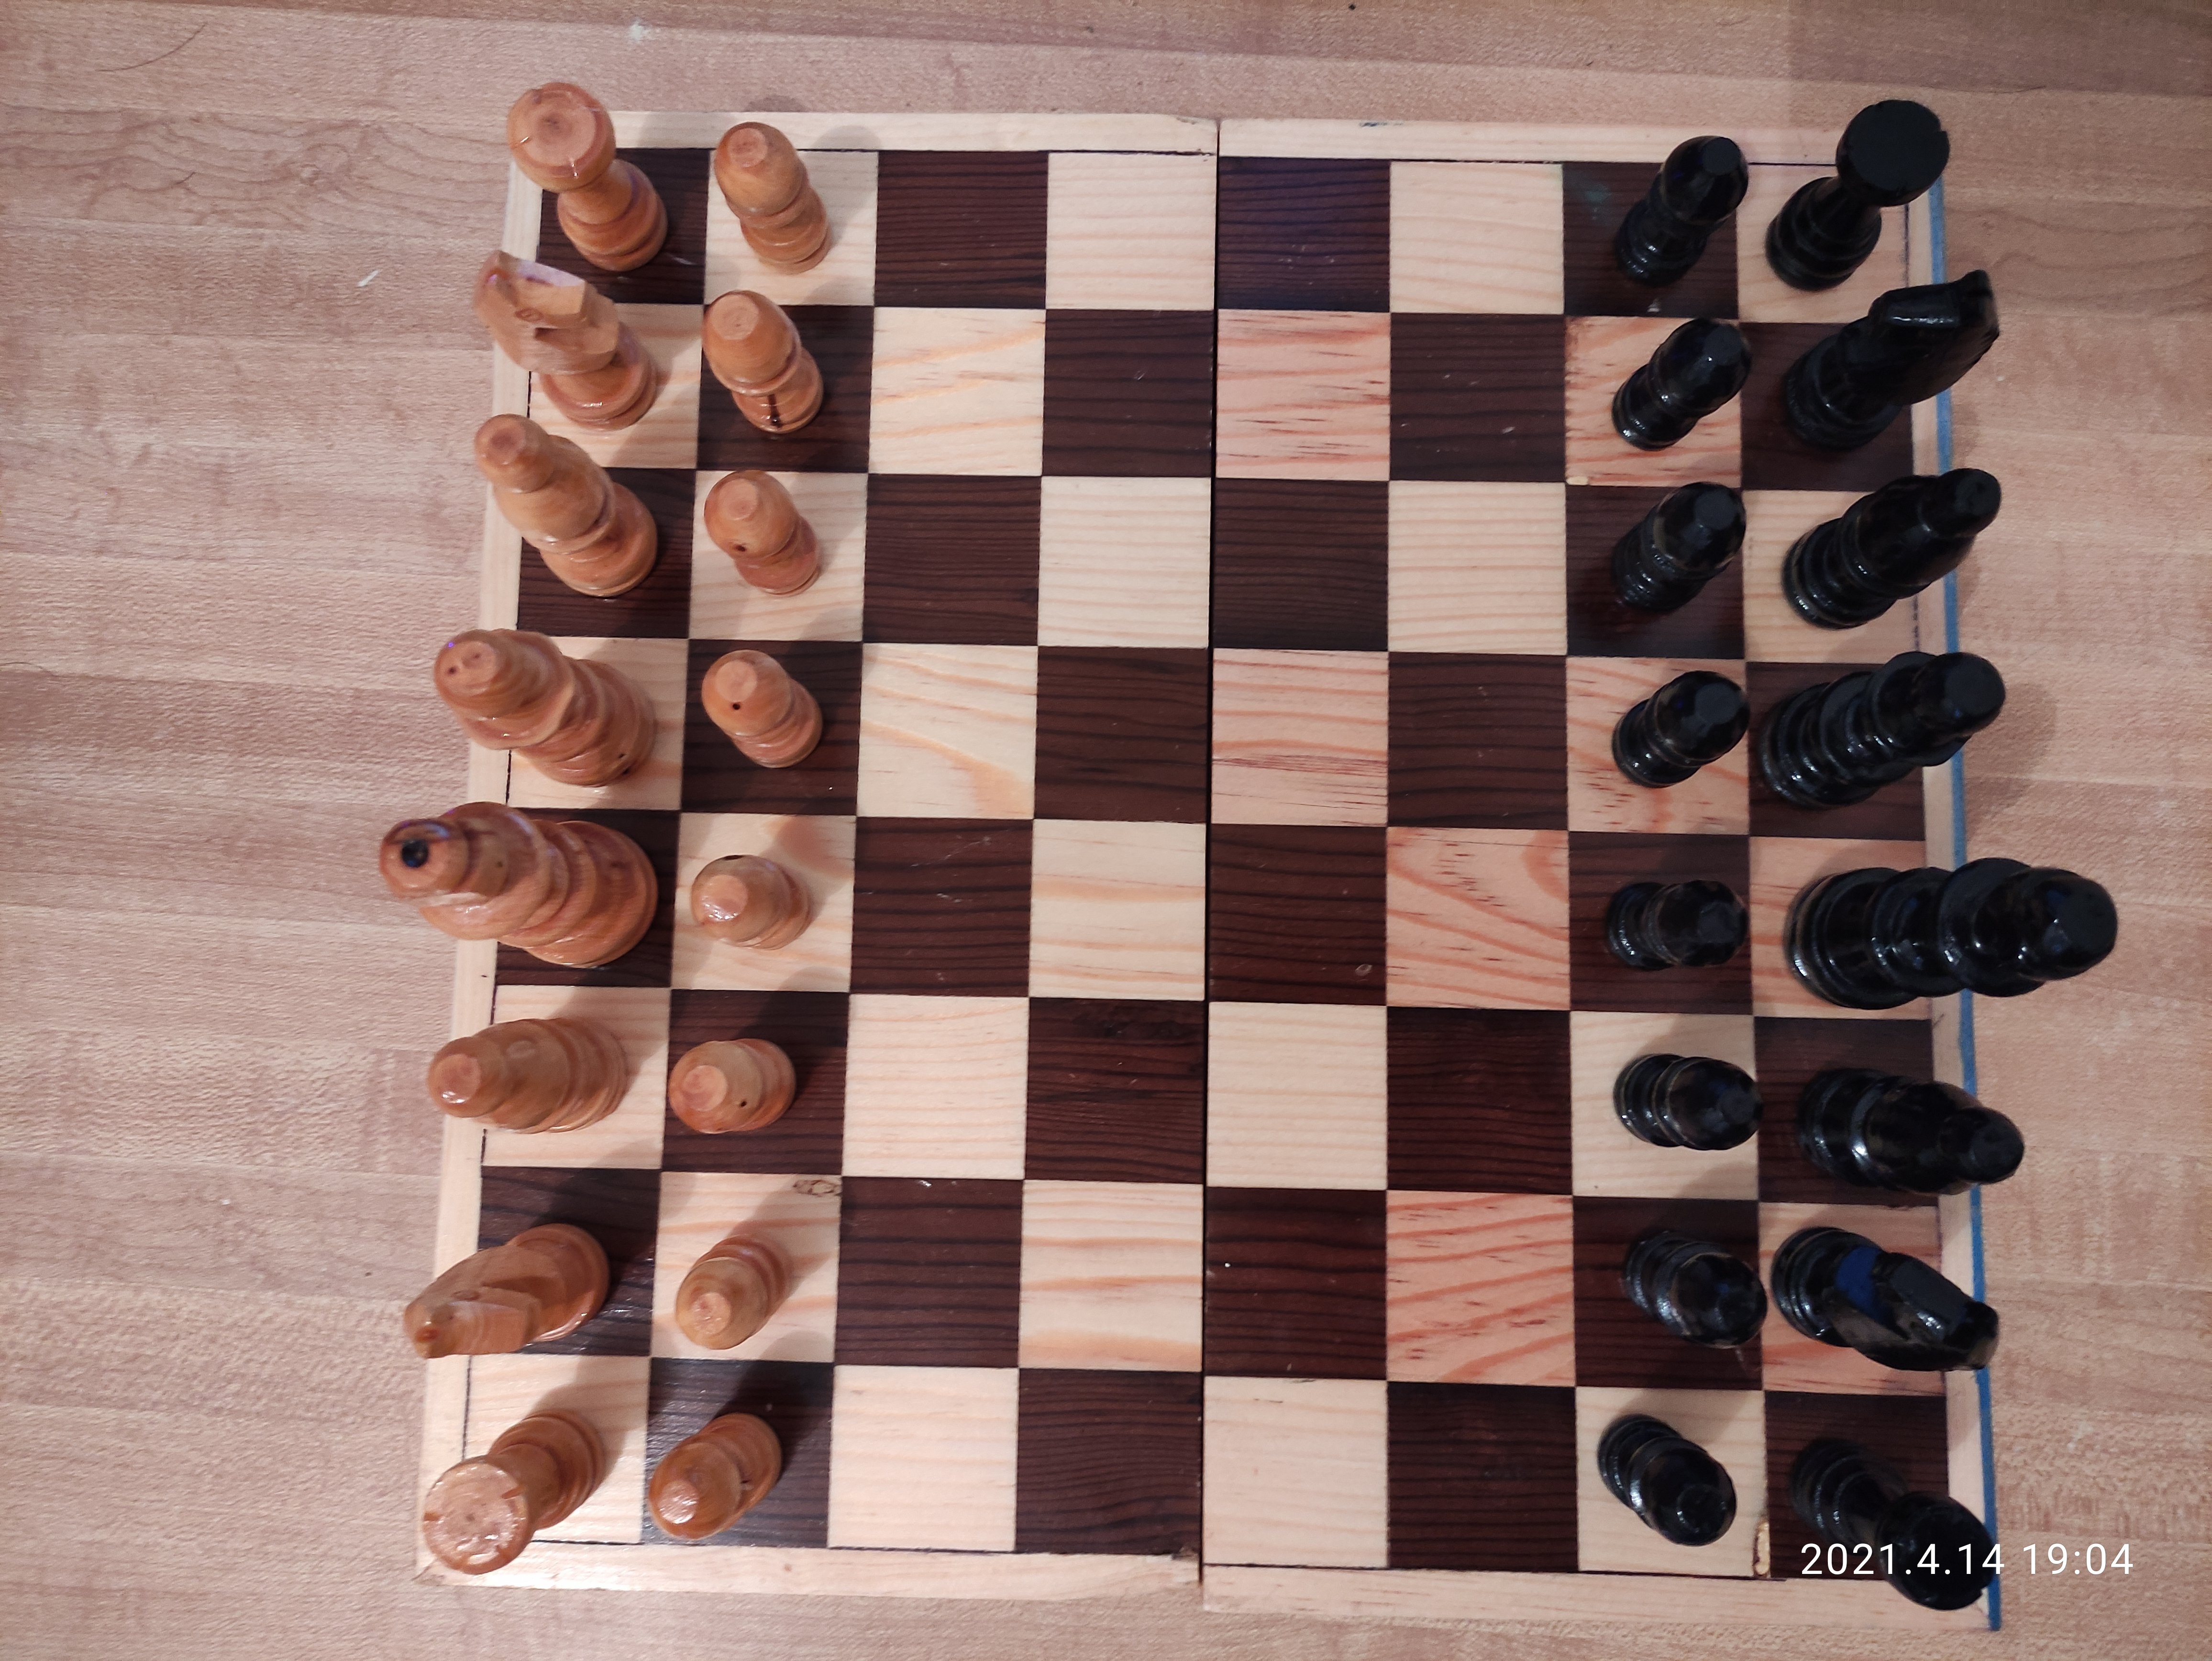
\includegraphics[width=0.75\textwidth]{Figs/AjedrezFroylan2}
     \end{center}
\end{column}

\end{columns}
%\end{block} 
\footnotetext{\fullcite{Froylan_VC_2021}}
%\footnotetext{Froylan Melquiades Wbario Martinez, \textbf{Seguidor de movimientos de Ajedrez}. Universidad Politécnica de Victoria, Informe técnico proyecto de asignatura “Visión por Computadora”, 2021.  En evaluación.}
%\\setcounter{footnote}{0}
\end{frame}

\begin{frame}{Detección de movimientos en un tablero de ajedrez (2)}
%\begin{block}{Detección de movimientos en un tablero de ajedrez (2)} 
\begin{columns}
\begin{column}{0.38\textwidth}
Aplicación de escritorio:
	\begin{itemize}
\item Una vez detectadas las regiones, se emplea un cronometro para determinar la diferencia entre dos instantaneas consecutivas
\item Problemas actuales: Iluminación, sombras, oclusiones
	\end{itemize}
\end{column}
\begin{column}{0.28\textwidth}
\begin{center}
     %%%%% this is a minipage, so \textwidth is already adjusted to the size of the column
     \includegraphics[width=0.79\textwidth]{Figs/AjedrezFroylan3}\\
%     \includegraphics[width=0.49\textwidth]{Figs/AjedrezFroylan4}
     \end{center}
\end{column}
\begin{column}{0.28\textwidth}
\begin{center}
     %%%%% this is a minipage, so \textwidth is already adjusted to the size of the column
%     \includegraphics[width=0.49\textwidth]{Figs/AjedrezFroylan3}\\
     \includegraphics[width=0.79\textwidth]{Figs/AjedrezFroylan4}
     \end{center}
\end{column}

\end{columns}
%\end{block} 
\end{frame}

